\section{METHODOLOGY}

\subsection{Methodology Overview}
\begin{frame}[t]{Methodology Overview}
    \begin{block}{Methodology Direction}
        The study follows a design and development methodology: review theory, design reusable architecture, implement the framework, and validate it through experiments.
    \end{block}
    % overall architecture workflow
    \begin{figure}[H]
        \centering
        \resizebox{\textwidth}{!}{%
            \begin{tikzpicture}[
                    node distance=2.2cm,
                    every node/.style={
                            draw,
                            fill=lightblue,
                            align=center,
                            rounded corners,
                            thick,
                            font=\large,
                            minimum width=4.2cm,
                            minimum height=2.0cm
                        }
                ]
                \node (r1) {Literature Review\\and Requirements Analysis};
                \node (r2) [right=of r1] {Software\\Architecture Design};
                \node (r3) [right=of r2] {Framework\\Construction};
                \node (r4) [right=of r3] {Experimental\\Validation};
                \node (r5) [right=of r4] {Deployment\\PyPi Package};
                \node (r6) [below=of r5, fill=mainblue, text=white] {Documentation};

                \draw[->] (r1) -- (r2);
                \draw[->] (r2) -- (r3);
                \draw[->] (r3) -- (r4);
                \draw[->] (r4) -- (r5);
                \draw[->] (r5) -- (r6);
            \end{tikzpicture}%
        }
    \end{figure}
\end{frame}

\subsection{KFCProcedure Architecture and Usage}
% =========================================================
% KFCProcedure Architecture
% =========================================================
\begin{frame}[fragile,t]{KFCProcedure Architecture}
    \footnotesize
    \vspace{-0.5cm}
    \begin{columns}[T,onlytextwidth]

        % =========================
        % Left: Architecture figure
        % =========================
        \column{0.50\textwidth}
        \centering
        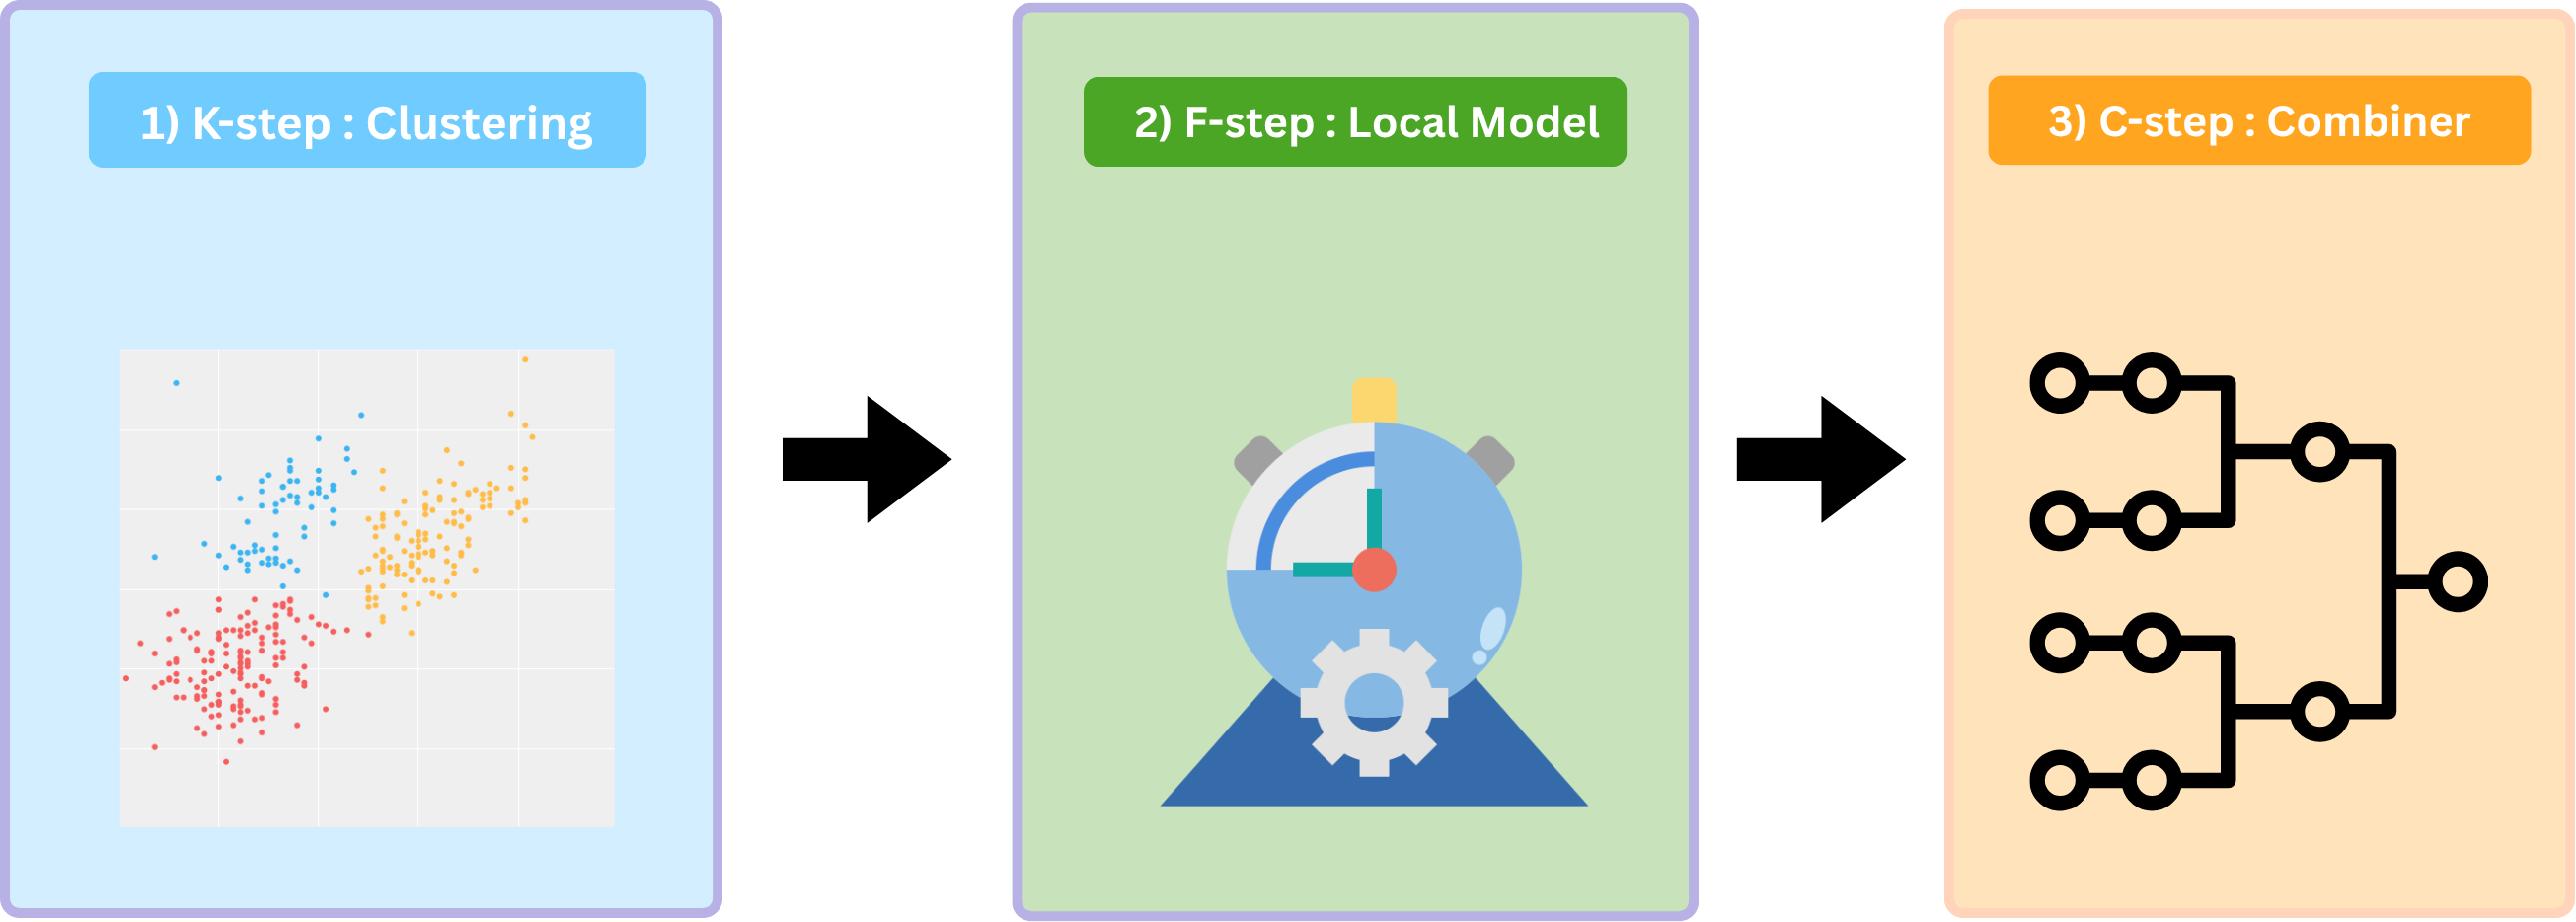
\includegraphics[
            width=\linewidth,
            height=4.45cm,
            keepaspectratio
        ]{figures/architectures/kfc.png}

        % =========================
        % Right: Engineering view
        % =========================
        \column{0.48\textwidth}

        \textbf{Engineering View}
        \vspace{0.10cm}

        \begin{itemize}
            \setlength\itemsep{0.13cm}

            \item Implemented as a \textbf{three-stage estimator}:
                  \[
                      \texttt{KStep} \rightarrow \texttt{FStep} \rightarrow \texttt{CStep}
                  \]

            \item Each stage is separated into reusable modules for clustering, local modeling, and aggregation.

            \item The \textbf{C-step} uses a configurable combiner through a factory-based design.

            \item Supports rule-based and learned combiners such as \texttt{mean}, \texttt{weighted\_mean}, \texttt{stacking}, and COBRA-based methods.
        \end{itemize}

    \end{columns}

    \vspace{0.25cm}

    \begin{block}{Implementation Purpose}
        KFCProcedure transforms clusterwise learning into a modular Python package where local models and aggregation strategies can be configured, replaced, and extended.
    \end{block}

\end{frame}

\begin{frame}[fragile, t]{KFCProcedure Usage}
    \vspace{-0.5cm}
    \begin{table}
        \scriptsize
        \renewcommand{\arraystretch}{1.2}
        \setlength{\tabcolsep}{1.8pt}
        \begin{tabularx}{\textwidth}{
                >{\raggedright\arraybackslash}m{2.55cm}
                >{\raggedright\arraybackslash}m{2.55cm}
                >{\raggedright\arraybackslash}X}
            \toprule
            \textbf{Parameter}          &
            \textbf{Required / Default} &
            \textbf{Purpose}                                                                 \\
            \midrule
            \texttt{divergences}        &
            \texttt{yes}                &
            List of Bregman divergences strings or instances for clustering.                 \\
            \texttt{local\_model}       &
            \texttt{yes}                &
            Base learner string or instance used for cluster-wise local modeling.            \\
            \texttt{combiner}           &
            \texttt{yes}                &
            Strategy algorithm handling ensemble aggregation.                                \\
            \texttt{task}               &
            \texttt{"regression"}       &
            Type of learning objective (\texttt{"regression"} or \texttt{"classification"}). \\
            \texttt{n\_clusters}        &
            \texttt{3}                  &
            Number of targeted clusters per divergence metric.                               \\
            \texttt{max\_iter}          &
            \texttt{300}                &
            Maximum iterations allowed for clustering optimization.                          \\
            \texttt{tol}                &
            \texttt{1e-4}               &
            Convergence numerical tolerance threshold.                                       \\
            \texttt{verbose}            &
            \texttt{0}                  &
            Debug logging depth configuration level (0 to 3).                                \\
            \texttt{random\_state}      &
            \texttt{None}               &
            Reproducibility random seed anchor.                                              \\
            \bottomrule
        \end{tabularx}
    \end{table}
    \tiny *Note: Additional parameters can be passed explicitly via \texttt{divergences\_params}, \texttt{local\_model\_params}, and \texttt{combiner\_params} dictionaries.
\end{frame}

\begin{frame}[fragile, t]{KFCProcedure Usage}
    \begin{minted}[
        fontsize=\scriptsize,
        breaklines,
        linenos,
        frame=single,
        framesep=2mm
    ]{python}
        from kfc_procedure import KFCProcedure

        model = KFCProcedure(
            divergences=["euclidean"], # euclidean, gkl, is, logistic
            local_model="lasso",       # linear_regression, ridge, lasso
            combiner="mean",           # mean
            task="regression",         # regression or classification
            n_clusters=3,              # number of clusters per divergence
            max_iter=300,              # maximum iterations for clustering
            tol=1e-4,                  # convergence numerical tolerance threshold.
            verbose=1,                 # debug logging level (0 to 3)
            random_state=42            # reproducibility random seed
        )
        model.fit(X_train, y_train)
        preds = model.predict(X_test)

    \end{minted}
\end{frame}

\subsection{COBRA-Baseed Aggregation}
\begin{frame}[t]{COBRA-Based Architecture}
    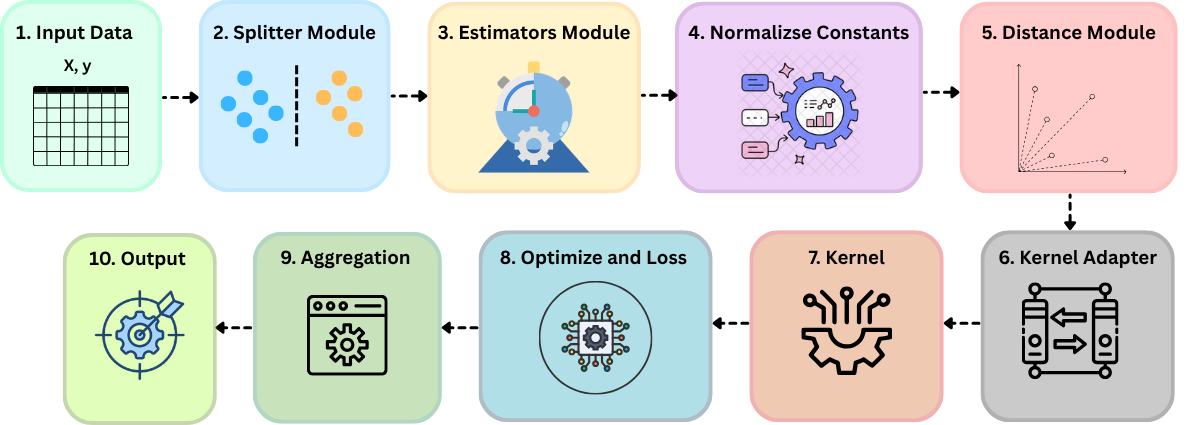
\includegraphics[width=\linewidth]{figures/architectures/gradientcobra.png}
\end{frame}

\begin{frame}[t]{COBRA-Based Usage}
    \vspace{-0.5cm}
    \begin{table}
        \scriptsize
        \renewcommand{\arraystretch}{1.2}
        \setlength{\tabcolsep}{1.8pt}
        \begin{tabularx}{\textwidth}{
                >{\raggedright\arraybackslash}m{2.55cm}
                >{\raggedright\arraybackslash}m{2.55cm}
                >{\raggedright\arraybackslash}X}
            \toprule
            \textbf{Parameter}          &
            \textbf{Required / Default} &
            \textbf{Purpose}                                                                          \\
            \midrule
            \texttt{estimators}         &
            \texttt{None}               &
            Base regressors; falls back to default if \texttt{None}.                                  \\
            \texttt{distance}           & \texttt{"euclidean"}      & Spatial closeness metric.       \\
            \texttt{kernel}             & \texttt{"rbf"}            & Proximity weighing engine.      \\
            \texttt{aggregator}         & \texttt{"weighted\_mean"} & Multi-expert combination logic. \\
            \texttt{loss}               & \texttt{"mse"}            & Optimization objective target.  \\
            \texttt{optimizer}          & \texttt{"grid"}           & Parameter search routine.       \\
            \texttt{learning\_rate}     & \texttt{0.1}              & Gradient adjustment step size.  \\
            \texttt{max\_iter}          & \texttt{300}              & Cap on optimizer updates.       \\
            \texttt{n\_cv}              & \texttt{5}                & Cross-validation folds.         \\
            \texttt{n\_jobs}            & \texttt{-1}               & CPU core allocation profile.    \\
            \bottomrule
        \end{tabularx}
    \end{table}
\end{frame}

\begin{frame}[fragile, t]{COBRA-Based Usage}
    \begin{minted}[
        fontsize=\scriptsize,
        breaklines,
        linenos,
        frame=single,
        framesep=2mm
    ]{python}
        from kfc_procedure.cobra import GradientCOBRA

        model = GradientCOBRA(
            estimators=["linear_regression", "random_forest_regressor"],
            kernel="rbf",           # weighting function
            distance="euclidean",   # prediction-space similarity
            loss="mse",             # optimization objective
            optimizer="grid",       # search or gradient
            max_iter=300,           # maximum iterations for optimization           
            n_cv=5,                 # cross-validation folds for hyperparameter tuning
            n_jobs=-1,              # CPU core allocation for parallel processing
            learning_rate=0.1,      # step size for gradient updates
            random_state=42,        # reproducibility random seed
        )
        model.fit(X_train, y_train)
        preds = model.predict(X_test)

    \end{minted}
\end{frame}

\subsection{Hybrid Workflow}
\begin{frame}[t]{Hybrid KFCProcedure and GradientCOBRA Workflow}
    \centering
    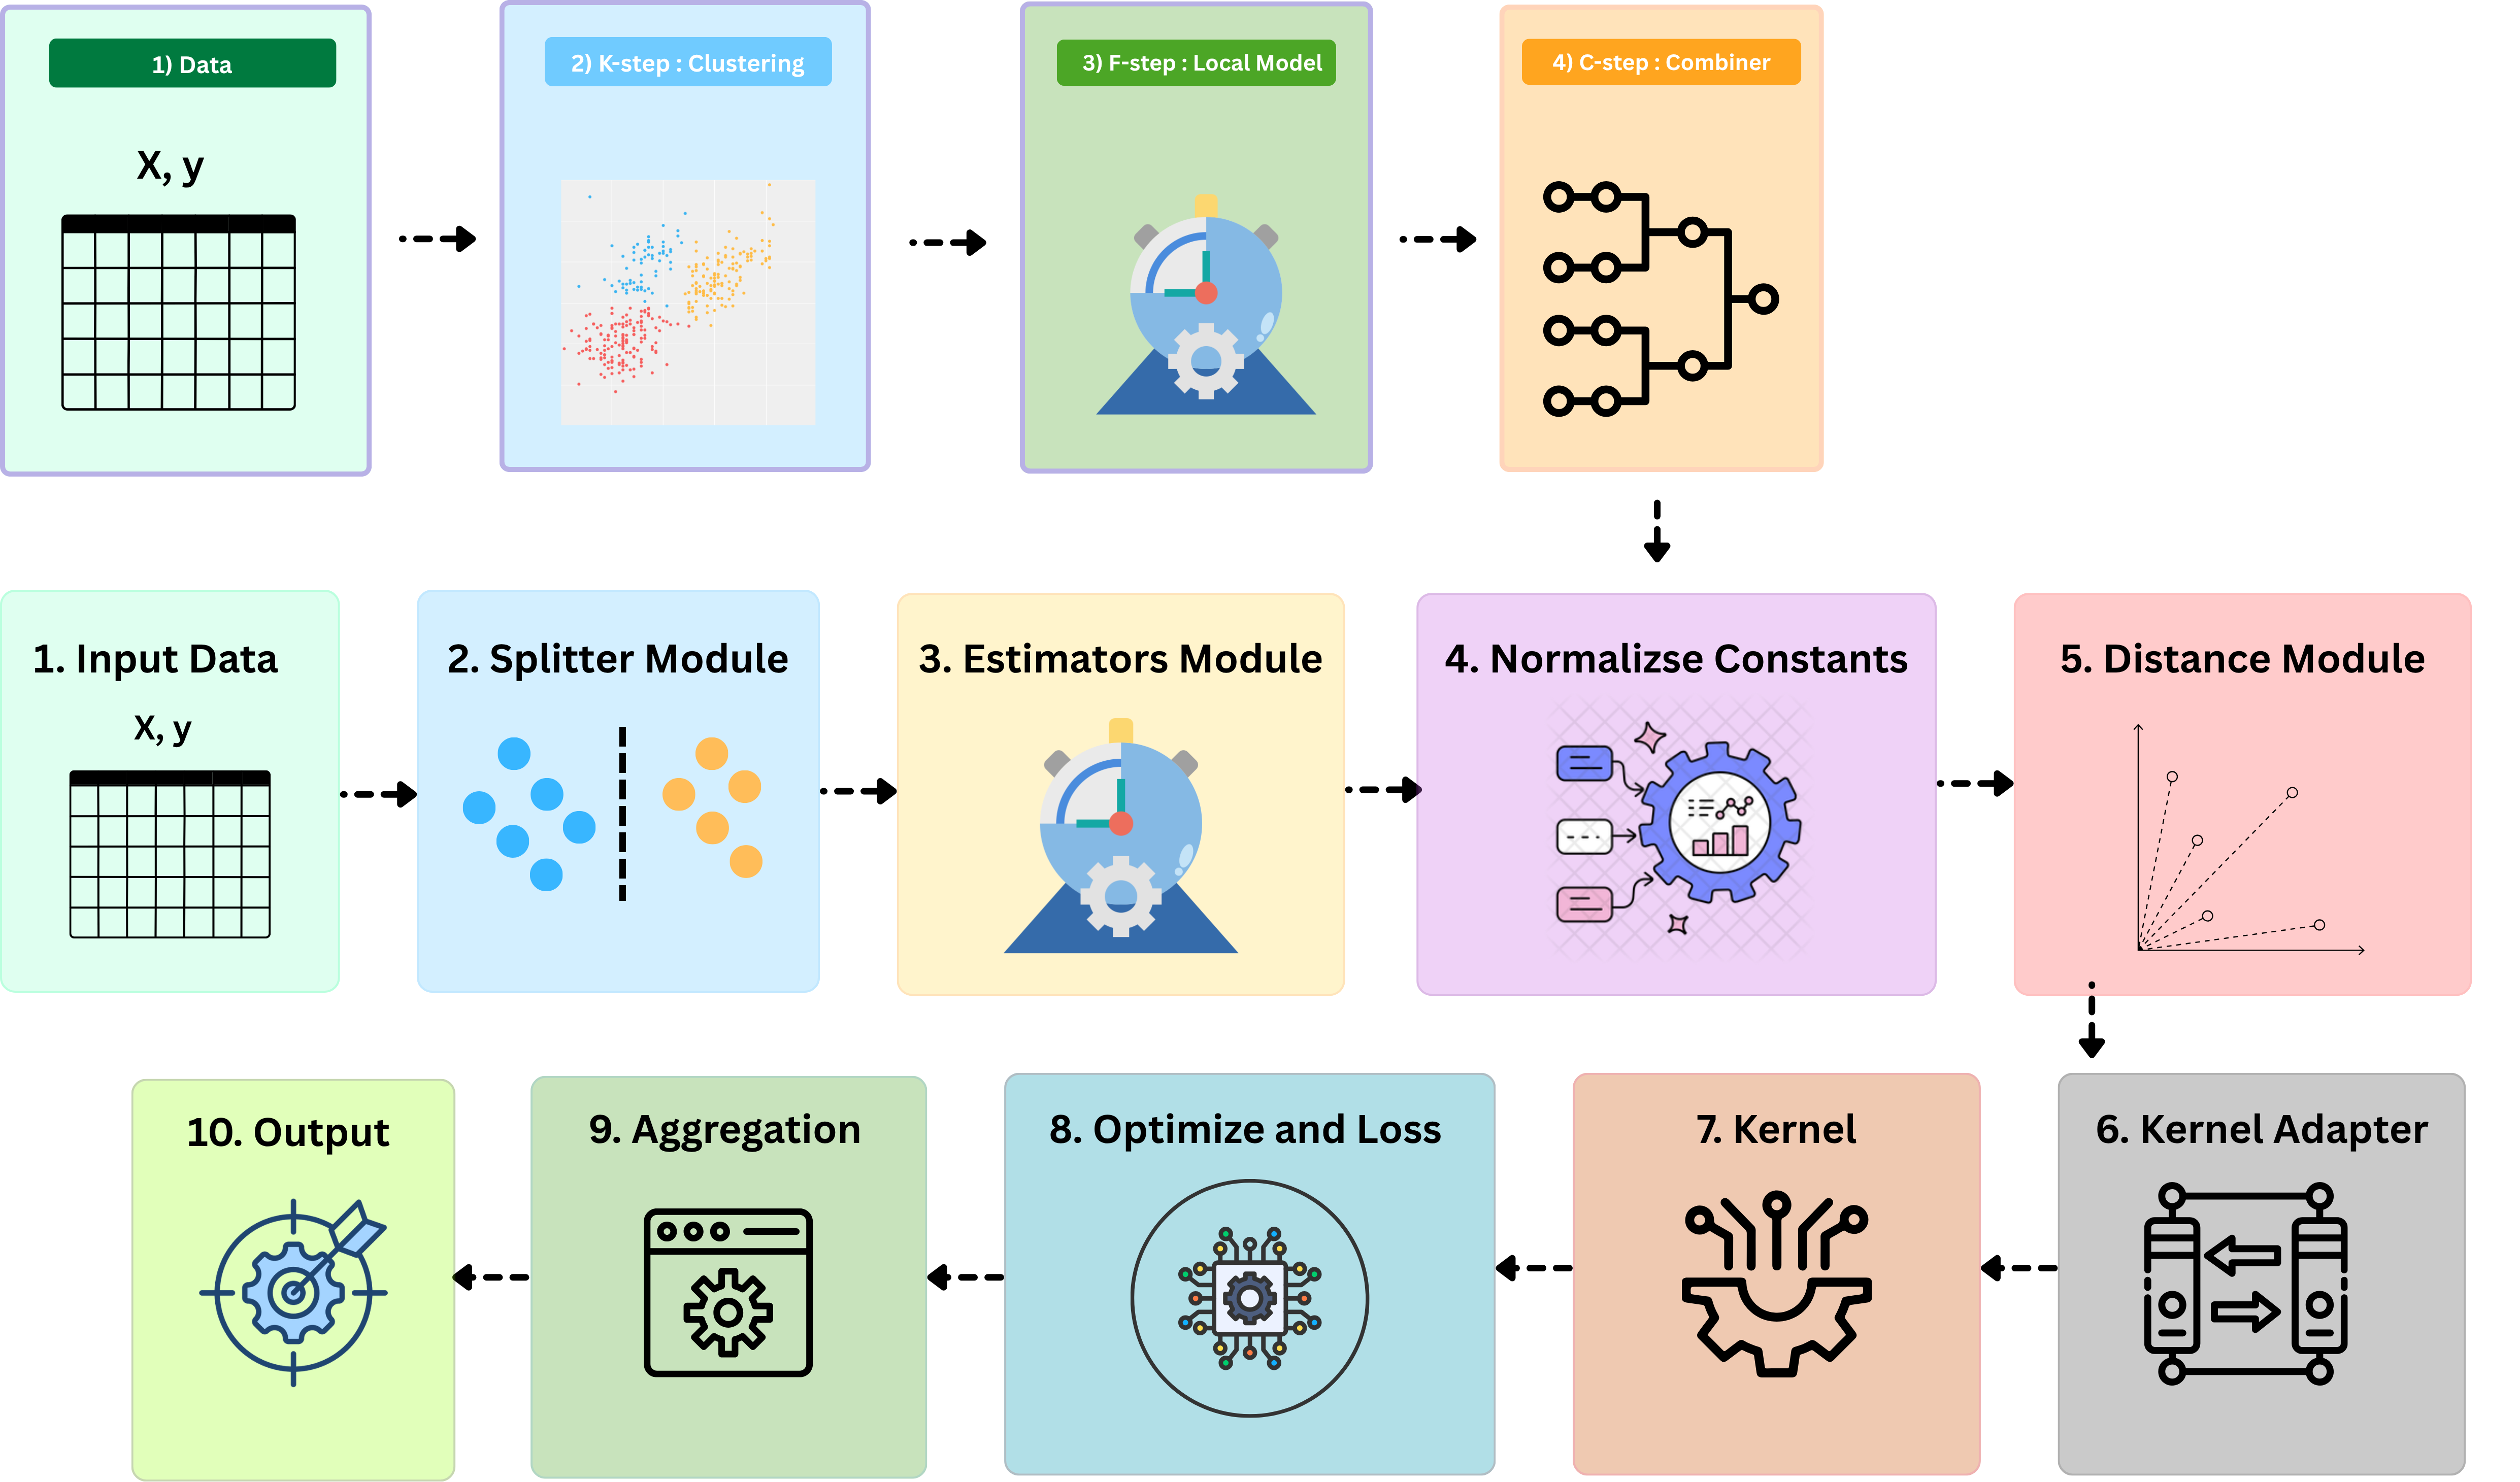
\includegraphics[height=6.5cm, width=0.8\textwidth]{figures/architectures/hybrid.png}
\end{frame}

\subsection{Modular and Extensible Design}

\begin{frame}[fragile,t]{Modular and Extensible Design}
    \footnotesize
    \vspace{-0.25cm}

    \begin{columns}[T,onlytextwidth]

        \column{0.43\textwidth}
        \textbf{Engineering Purpose}
        \vspace{0.12cm}

        \begin{itemize}
            \setlength\itemsep{0.18cm}

            \item \textbf{Configurable C-step:}
                  aggregation methods can be changed without changing the full KFCProcedure workflow.

            \item \textbf{Plug-in design:}
                  new combiners can be added and registered by name.

            \item \textbf{Reusable package structure:}
                  clustering, local modeling, and aggregation are separated into modules.

            \item \textbf{Maintainability:}
                  custom logic stays outside the core pipeline, reducing future modification risk.
        \end{itemize}

        \column{0.55\textwidth}
        \textbf{Example: Adding a New C-Step Combiner}
        \vspace{0.08cm}

        \begin{minted}[
            fontsize=\tiny,
            breaklines,
            frame=single,
            framesep=0.3mm,
            xleftmargin=0pt,
            xrightmargin=0pt,
            autogobble
        ]{python}
            from kfc_procedure import KFCRegressor
            from kfc_procedure.combiners import BaseCombiner, CombinerFactory
            import numpy as np

            @CombinerFactory.register("median", categories={"regression"})
            class MedianCombiner(BaseCombiner):
                def fit(self, X, y=None):
                    return self

                def combine(self, X):
                    return np.median(X, axis=1)

            model = KFCRegressor(
                divergences=["euclidean", "gkl"],
                local_model="linear_regression",
                combiner="median"
            )
        \end{minted}

    \end{columns}

    \vspace{0.12cm}

    \begin{block}{Key Benefit}
        \scriptsize
        New aggregation strategies can be added as plug-ins, while the main KFCProcedure pipeline remains unchanged.
    \end{block}

\end{frame}